\section{Negativ återkoppling}

\paragraph{Vad är negativ återkoppling?}
I denna kursen kommer vi huvudsakligen att studera hur man kontrollerar ett system vid att låta avvikelsen mot det önskade värdet kontrollera regleringen av storheten, alltså låta $U = FE$, där $e = r - y$.

\paragraph{Illustration i blockdiagram}
Ett enkelt negativt återkopplad system illustrearas i figur \ref{fig:negative_feedback}.
\begin{figure}[!ht]
	\centering
	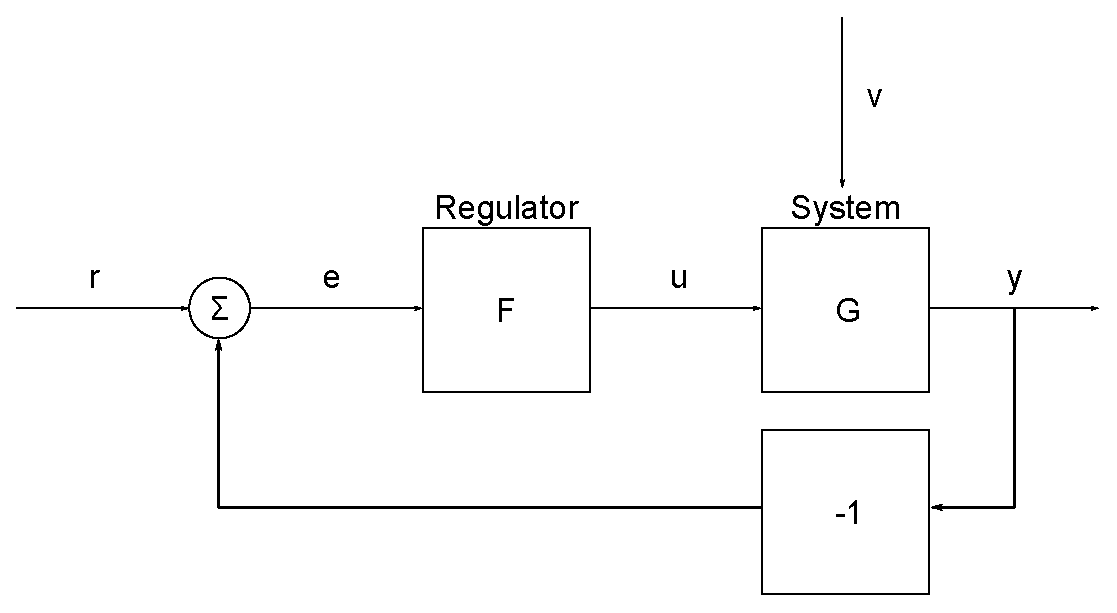
\includegraphics[width = \textwidth]{./Images/negative_feedback.eps}
	\caption{Schematisk illustration av ett enkelt negativt återkopplad system.}
	\label{fig:negative_feedback}
\end{figure}

\paragraph{Beskrivning av systemet}
Vi börjar beskrivningen av systemet med att inte betrakta störningar. I ena ändpunkten har vi
\begin{align*}
	Y = GU = GFE.
\end{align*}
Summationskomponenten till vänster ger oss
\begin{align*}
	E = R - Y,
\end{align*}
och därmed
\begin{align*}
	Y = GFR - GFY.
\end{align*}
Därmed kan vi skriva
\begin{align*}
	Y = \frac{GF}{1 + GF}R.
\end{align*}

\paragraph{Återkopplad överföringsfunktion}
För ett återkopplad system som kan skrivas som $Y = G_{\text{C}}R$ definieras $G_{\text{C}}$ som den återkopplade överföringsfunktionen. För systemet ovan har vi alltså
\begin{align*}
	G_{\text{C}} = \frac{GF}{1 + GF}R.
\end{align*}

\paragraph{Samband mellan reglerfel och referens}
Alternativt kan vi lösa systemet ovan för att få
\begin{align*}
	R - E = GFE,\ E = \frac{1}{1 + GF}R.
\end{align*}

\paragraph{Samband mellan referens och styrsignal}
Systemet ovan kan även lösas för att ge
\begin{align*}
	U = FR - FY = FR - GFU,\ U = \frac{F}{1  + GF}R.
\end{align*}

\paragraph{Slutna systems poler}
Vi ser att slutna system har poler där $1 + GF = 0$. Därmed bestäms systemets stabilitet av systemet och regulatorn.

\paragraph{P-reglering}
Principet i P-reglering är att välja en styrsignal som är proportionell mot storleken av felet, alltså
\begin{align*}
	u = K(r - y) = Ke.
\end{align*}
Det är här klart att för att få negativ återkoppling väljer vi $K > 0$.

Denna regleringsmetoden
\begin{itemize}
	\item minskar inverkan av störning och modellfel för ett bra val av $K$.
	\item ökar snabbheten vid insvängning.
	\item stabiliserar instabila system.
\end{itemize}
Däremot kan regleringen gå fel om t.ex.
\begin{itemize}
	\item systemet inte uppför sig som man tror.
	\item man har begränsningar i styrförmåga.
	\item man får instabilitet på grund av återkopplingen.
\end{itemize}

Det är även ett problem att om felet är stationärt, är även styrsignalen det, så även om du har ett nollskild fel klarar inte systemet nödvändigtvis anpassa sig.

\paragraph{PID-reglering}
PID står för proportionell integrerande deriverande. Denna sortens reglering löser många reglerproblem. Med PID-reglering väljer vi styrsignlaen
\begin{align*}
	u = K_{\text{P}}e + K_{\text{I}}\integ{t_{0}}{t}{\tau}{e} + K_{\text{D}}\dv{e}{t}.
\end{align*}
Alternativt kan vi skriva det som
\begin{align*}
	u = K\left(e + \frac{1}{T_{\text{I}}}\integ{t_{0}}{t}{\tau}{e} + T_{\text{D}}\dv{e}{t}\right).
\end{align*}

De tre ingående termerna i styrsignalen är
\begin{itemize}
	\item proportionell återkoppling, som betraktar det nuvarande felet.
	\item integrerande återkoppling, som betraktar hur felet har uppfört sig.
	\item deriverande återkoppling, som betraktar hur felet kommer att uppföra sig.
\end{itemize}

\paragraph{PI-reglering}
PI-reglering använder ej den deriverande återkopplingstermen. Vi ser härifrån att vid ett stationärt tillstånd är antingen $e = 0$, annars ökar eller minskar $u$ på grund av integraltermen.

Vi vill nu betrakta systemets insvängning. Om det stationära $\bar{u}$ krävs för att $e = 0$, har vi
\begin{align*}
	\bar{u} = K\left(e + \frac{1}{T_{\text{I}}}\integ{t_{0}}{t}{\tau}{e}\right).
\end{align*}
Vid att derivera detta fås
\begin{align*}
	K\left(\dv{e}{t} + \frac{1}{T_{\text{I}}}e\right) = 0,
\end{align*}
med lösning proportionell mot $e^{-\frac{t}{T_{\text{I}}}}$.

Notera att om man har stort fel kan PI-reglering ge problem. Därför använder man det typiskt när felen är små.

\paragraph{PI-reglering i Laplacevärlden}
Vid att Laplacetransformera uttrycket för styrsignalen i en PI-regulator, nämligen
\begin{align*}
	u = K\left(e + \frac{1}{T_{\text{I}}}\integ{t_{0}}{t}{\tau}{e}\right),
\end{align*}
fås
\begin{align*}
	U = K\left(E + \frac{1}{T_{\text{I}}s}E\right),
\end{align*}
och därmed
\begin{align*}
	F(s) = K\left(1 + \frac{1}{T_{\text{I}}s}\right).
\end{align*}

\paragraph{Rotorter med negativt återkopplade system}
Betrakta ett system med överförningsfunktion $G_{\text{O}}$ för det öppna systemet. Det slutna systemet kommer ha överförningsfunktion
\begin{align*}
	G_{\text{C}} = \frac{G_{\text{O}}}{1 + G_{\text{O}}}.
\end{align*}
$G_{\text{O}}$ är ofta på formen
\begin{align*}
	G_{\text{O}} = K\frac{Q}{P},
\end{align*}
där $K$ är en parameter. Då får vi
\begin{align*}
	G_{\text{C}} = \frac{KQ}{P + KQ}.
\end{align*}
Systemet har alltså poler som ges av
\begin{align*}
	P + KQ = 0,\ \frac{P}{Q} = -K.
\end{align*}
Detta kriteriet anger systemets rotort.

\paragraph{Hur man ritar rotorter}
Vi antar nu att $P$ och $Q$ är polynom av grad $n$ respektiva $m$, där $n \geq m$. Då vet vi att kriteriet har $n$ rötter, och rotorten har därför $n$ grenar (annars skulle den inte kunna starta i $n$ punkter).

Rötterna dyker antingen upp som reellvärda eller i par av komplexkonjugerade rötter, och därmed är rotorten symmetrisk med avseende på reella axeln. Vi vet även att rotorten har $n - m$ asymptoter, då det bara finns $m$ ändpunkter.

Det gäller även att alla delar av reella axeln som har ett udda antal reella start- och ändpunkter till höger om sig tillhör rotorten. För att förstå detta, faktorisera polynomen på vänstersidan och para ihop de komplexkonjugerade paren så att alla koefficienter är reella. Om man startar långt till höger på reella axeln är kvoten positivt, och tillhör ej rotorten. Varje gång den passerar en start- eller ändpunkt byter kvoten tecken, och den kan då tillhöra rotorten. En bra matteövning kan vara att övertyga sig om att det även är sant för de komplexa nollställen.

Vi vill nu studera asymptoterna, och antar därför här att $n > m$. Vi skriver då
\begin{align*}
	\frac{P}{Q} = \frac{s^{n} + a_{1}s^{n - 1} + \dots}{s^{m} + b_{1}s^{m - 1} + \dots} = s^{n - m} + (a_{1} - b_{1})s^{n  - m - 1} + \frac{P_{1}}{Q}.
\end{align*}
Vi använder binominalsatsen för att skriva
\begin{align*}
	\frac{P}{Q} = \left(s + \frac{a_{1} - b_{1}}{n - m}\right)^{n - m} + \frac{P_{2}}{Q},
\end{align*}
där utvecklingen av parentesen kommer återskapa de två potenstermerna ovan. $P_{2}$ har grad $n - 2$, så för $s$ med stora belopp kommer parentesen dominera. Rotortkriteriet ger
\begin{align*}
	\arg\left(s + \frac{a_{1} - b_{1}}{n - m}\right) = \frac{\pi}{n - m} + \frac{2\pi}{n - m}k,\ k = 0, \dots, m - n.
\end{align*}
Detta är strålar från punkten $-\frac{a_{1} - b_{1}}{n - m}$ som pekar i riktningerna $\frac{\pi}{n - m} + \frac{2\pi}{n - m}k$ för stora $s$. Eftersom asymptoterna strålar ut från denna punkten, ser vi att den är rotortens centroid. Binominalsatsen ger även att $a_{1}$ är summan av systemets poler och $b_{1}$ är summan av systemets nollställen.

Det finns en entydighetssats för rotortkriteriet, vilket innebär att om det finns en del av reella axeln mellan två poler som är med i rotorten, kommer rotorten behöva bryta ut från reella axeln någonstans imellan dessa två polerna. På samma sättet kommer rotorten bryta in i reella axeln i områden mellan två nollställen som är med i rotorten.

Om man vill, kan man räkna ut vinkeln i punkterna där rotorten bryter in och ut. Detta vet jag dock inte hur man gör. Man kan även räkna ut för vilka $s$ rotorten bryter in och ut. För att göra detta, ställ upp karakteristiska ekvationen $P + KQ = 0$, derivera med avseende på $s$. Punkterna som uppfyller $\dv{K}{s} = 0$ som ger $K > 0$ är punkterna där rotorten bryter in och ut.

För att rita rotorten kan du följa dessa steg:
\begin{itemize}
	\item Beräkna överförningsfunktionen för det slutna systemet. Skriv nämnaren som $P + KQ = 0$.
	\item Hitta startpunkterna, alltså rötterna till $P$.
	\item Hitta ändpunkterna, alltså rötterna till $Q$.
	\item Bestäm antal asymptoter, alltså gradtalet till $P$ minus gradtalet till $Q$.
	\item Bestäm vilka delar av reella axeln som tillhör rotorten. Det är de delar som har ett udda antar start- och slutpunkter till höger om sig.
	\item Beräkna punkterna där rotorten korsar reella axeln. Såna ligger mellan två startpunkter. För att hitta dem kan man ansätta att karakteristiska ekvationen har en dubbelrot, och identifiera vilka kombinationer av $s$ och $K$ som ger detta, eller hitta stationära punkter  för $K$ som funktioner av $s$.
	\item Bestäm centroiden $-\frac{\sum p_{i} - \sum q_{i}}{n - m}$, där $p_{i}$ är systemets poler och $q_{i}$ dets nollställen.
	\item Bestäm asymptoternas riktningar relativt centroiden genom att betrakta argumentet till $\frac{P}{Q} = -K$ för stora $s$. Spoilers: De är $\frac{\pi}{n - m} + \frac{2\pi}{n - m}k,\ k = 0, \dots, m - n$.
	\item Bestäm korsningar med imaginära axeln genom att sätta $s = i\omega$. Kom ihåg att $K\geq 0$.
	\item Rita.
\end{itemize}

\paragraph{Nyquistkurvan}
Givet överförningsfunktionen
\begin{align*}
	G_{\text{C}} = \frac{G_{\text{O}}}{1 + G_{\text{O}}}.
\end{align*}
för ett slutet system, finns det några poler så att systemet är instabilt? En ide för att undersöka detta är att undersöka alla $s$ i högre halvplan och se vilka värden på $G_{\text{O}}$ man får. Detta gör vi genom att rita två halvcirklar med radier $r$ respektivar $R$ i högre halvplan, förbinda dem med raka linjer i änderna och låta $r$ gå mot $0$ och $R$ mot $\infty$. $G_{\text{O}}$ kommer då anta värden på en kurva som kallas för Nyquistkurvan.

Eftersom Nyquistkurvan i stort sett antingen skickas mot oändligheten eller mot origo, är den viktigaste delen av Nyquistkurvan som är avbildad från imaginära axeln. Man kan även observera att $G_{\text{O}}(\infty) = 0$ och $G_{\text{O}}(0)\approx\frac{K}{s^{p}}$, där $p$ är antal poler i origo.

\paragraph{Nyquistkriteriet}
Betrakta ett öppet systems Nyquistkurva. Argumentvariationsprincipen från komplex analys ger oss att antalet poler i höger halvplan till ett återkopplad system är lika med antalet poler i höger halvplan hos $G_{\text{O}}$ plus antalet varv som Nyquistkurvan omsluter punkten $-1$. Detta kallas Nyquistkriteriet.

Speciellt, om $G_{\text{O}}$ inte har poler i höger halvplan, är systemet stabilt om Nyquistkurvan inte omsluter $-1$. Detta är varianten av Nyquistkriteriet som ofta används i denna kursen.